\documentclass[a4paper,12pt]{article}

\usepackage[T2A]{fontenc}			
\usepackage[utf8]{inputenc}			
\usepackage[english,russian]{babel}	

\usepackage[
bookmarks=true, colorlinks=true, unicode=true,
urlcolor=black,linkcolor=black, anchorcolor=black,
citecolor=black, menucolor=black, filecolor=black,
]{hyperref}

\usepackage{color}
\usepackage{caption}
\DeclareCaptionFont{white}{\color{black}}
\DeclareCaptionFormat{listing}{\colorbox{white}{\parbox{\textwidth}{#1#2#3}}}
\captionsetup[lstlisting]{format=listing,labelfont=white,textfont=white}

\usepackage{amsmath,amsfonts,amssymb,amsthm,mathtools} 
\usepackage{wasysym}

\usepackage{graphicx}
%\usepackage[cache=false]{minted}
\usepackage{cmap}
\usepackage{indentfirst}

\usepackage{listings} 
\usepackage{fancyvrb}

\usepackage{geometry}
\geometry{left=2cm}
\geometry{right=1.5cm}
\geometry{top=1cm}
\geometry{bottom=2cm}

\setlength{\parindent}{5ex}
\setlength{\parskip}{0.5em}

\usepackage{pgfplots}

\usepackage{longtable}

\begin{document}
	\lstset{ %
		language=C,                 % выбор языка для подсветки (здесь это С)
		basicstyle=\small\sffamily, % размер и начертание шрифта для подсветки кода
		numbers=left,               % где поставить нумерацию строк (слева\справа)
		numberstyle=\tiny,           % размер шрифта для номеров строк
		stepnumber=1,                   % размер шага между двумя номерами строк
		numbersep=5pt,                % как далеко отстоят номера строк от подсвечиваемого кода
		backgroundcolor=\color{white}, % цвет фона подсветки - используем \usepackage{color}
		showspaces=false,            % показывать или нет пробелы специальными отступами
		showstringspaces=false,      % показывать или нет пробелы в строках
		showtabs=false,             % показывать или нет табуляцию в строках
		frame=single,              % рисовать рамку вокруг кода
		tabsize=2,                 % размер табуляции по умолчанию равен 2 пробелам
		captionpos=t,              % позиция заголовка вверху [t] или внизу [b] 
		breaklines=true,           % автоматически переносить строки (да\нет)
		breakatwhitespace=false, % переносить строки только если есть пробел
		escapeinside={\%*}{*)}   % если нужно добавить комментарии в коде
	}
	
	% Титульный лист
	\begin{figure}[h!]
		\begin{center}
			{
\includegraphics[scale = 0.4]{titul.jpg}}
			\label{titul}
		\end{center}
	\end{figure}
	
	\vspace*{15mm} 
	
	\huge
	\begin{center}
		Дисциплина: <<Моделирование>>
	\end{center}
	
	\begin{center}
		Лабораторная работа №1
	\end{center}

	
	\huge
	\begin{center}
		Тема работы:\\
		<<Исследование псевдослучайных чисел>>
	\end{center}
	\vspace*{25mm} 
	
	\large
	\begin{flushright}
		Студент: Левушкин И. К. \\
		Группа: ИУ7-72Б \\
		Преподаватель: Рудаков И. В. \\
	\end{flushright}
	
	\vspace*{25mm}
	\begin{center}
		Москва, 2020 г.  
	\end{center}
	\thispagestyle{empty}
	
	
	\newpage
	
	\section*{Задание}
	
	Реализовать критерий оценки случайности последовательности. 
	
	Сравнить результаты работы данного критерия на одноразрядных, двухразрядных и трехразрядных последовательностях псевдослучайных целых чисел.
	
	Последовательности получать алгоритмическим способом и табличным способом.
	
	\section*{Формализация}
	
	\subsection*{Реализация последовательностей случайных последовательностей}
	
	В данной лабораторной работе генерация псевдослучайных чисел осуществляется с помощью вихря Мерсенна ~\cite{mersen}, табличные значения берутся из трёх файла.
	
	\subsection*{Критерий оценки случайности последовательности}
	
	В качестве критерия проверки случайности последовательности был выбран критерий равномерности (критерий частот), использующий $\chi^2$-критерий ~\cite{knut}. 
	
	Кратко описать данный критерий можно следующим образом:
	
	\begin{itemize}
		\item Пусть $k$ – количество всех возможных принимаемых значений, 
		
		\item $p_s$ - вероятность того, что наблюдение относится к категории $s$,
		
		\item $n$ - количество проведенных экспериментов,
		
		\item $Y_s$ - число экспериментов относящихся к категории $s$.
	\end{itemize}

	Поскольку все возможные принимаемые значения должны быть равновероятны, то $p_s = \frac{1}{k}$
	
	Тогда получим статистику $V$, также известную как расстояние Пирсона $D$:
	
	\[
	V = \frac{k}{n}\sum_{s = 1}^{k}\left(Y_s^2\right) - n
	\]
	
	Если V равно нулю, то распределение абсолютно равномерно, то есть все возможные принимаемые значения входят в анализируемую последовательность по одному разу.
	
	
	Для определения <<приемлемого>> значения $V$ используются значения из $\chi^2$-распределения с $\nu = k - 1$ степенями свободы:
	
	\begin{center}
		\begin{longtable}[h!]{|p{0.1\linewidth}|p{0.1\linewidth}|p{0.1\linewidth}|p{0.1\linewidth}|p{0.1\linewidth}|p{0.1\linewidth}|p{0.1\linewidth}|p{0.1\linewidth}|}
			\hline
			{} & {p = 1\%} & {p = 5\%} & {p = 25\%} & {p = 50\%} & {p = 75\%} & {p = 95\%} & {p = 99\%}\\
			\hline
			{$\nu = 9$} & {2.088} & {3.325} & {5.899} & {8.343} & {11.39} & {16.92} & {21.67}\\
			\hline
			{$\nu = 89$} & {60.93} & {68.25} & {79.68} & {88.33} & {97.60} & {112.02} & {122.94}\\
			\hline
			{$\nu = 899$} & {803.31} & {830.41} & {870.05} & {898.33} & {927.23} & {969.86} & {1000.57}\\
			\hline
			\caption{}
		\end{longtable}
	\end{center}

	Если в таблице выбрать число $x$, стоящее на $\nu$-ой строке и в столбце $p$, то это означает, что вероятность того, что значение $V$ будет меньше либо равно $x$, равно $x$, приближенно равна $p$, если $n$ достаточно велико.
	
	Чтобы определить насколько большим должно быть $n$, воспользуемся эмпирическим правилом:
	
	\textit{Необходимо взять n настолько большим, чтобы все значения величин $n p_s$ были больше или равны пяти.}
	
	В нашем случае $p_s$ равно:
	
	\begin{itemize}
		\item $\frac{1}{10} = 0.1$ при $k = 10$
		\item $\frac{1}{90} = 0.0(1)$ при $k = 90$
		\item $\frac{1}{900} = 0.00(1)$ при $k = 900$
	\end{itemize}

	В соответствии с сформулированным эмпирическим правилом необходимо провести $n >= 50$, $n >= 450$, $n >= 4500$ наблюдений для одноразрядных, двухразрядных и трехразрядных чисел, соответственно.
	
	В данной лабораторной работе используется $n = 100$, $n = 1000$, $n = 10000$ наблюдений для одноразрядных, двухразрядных и трехразрядных чисел, соответственно.
	
	\newpage
	
	\section*{Результаты работы}
	
	Ниже приведены результаты работы программы. В таблицах представлены первые 10 полученных чисел.
	
	\begin{figure}[h!]
		\begin{minipage}[b]{0.5\textwidth}
			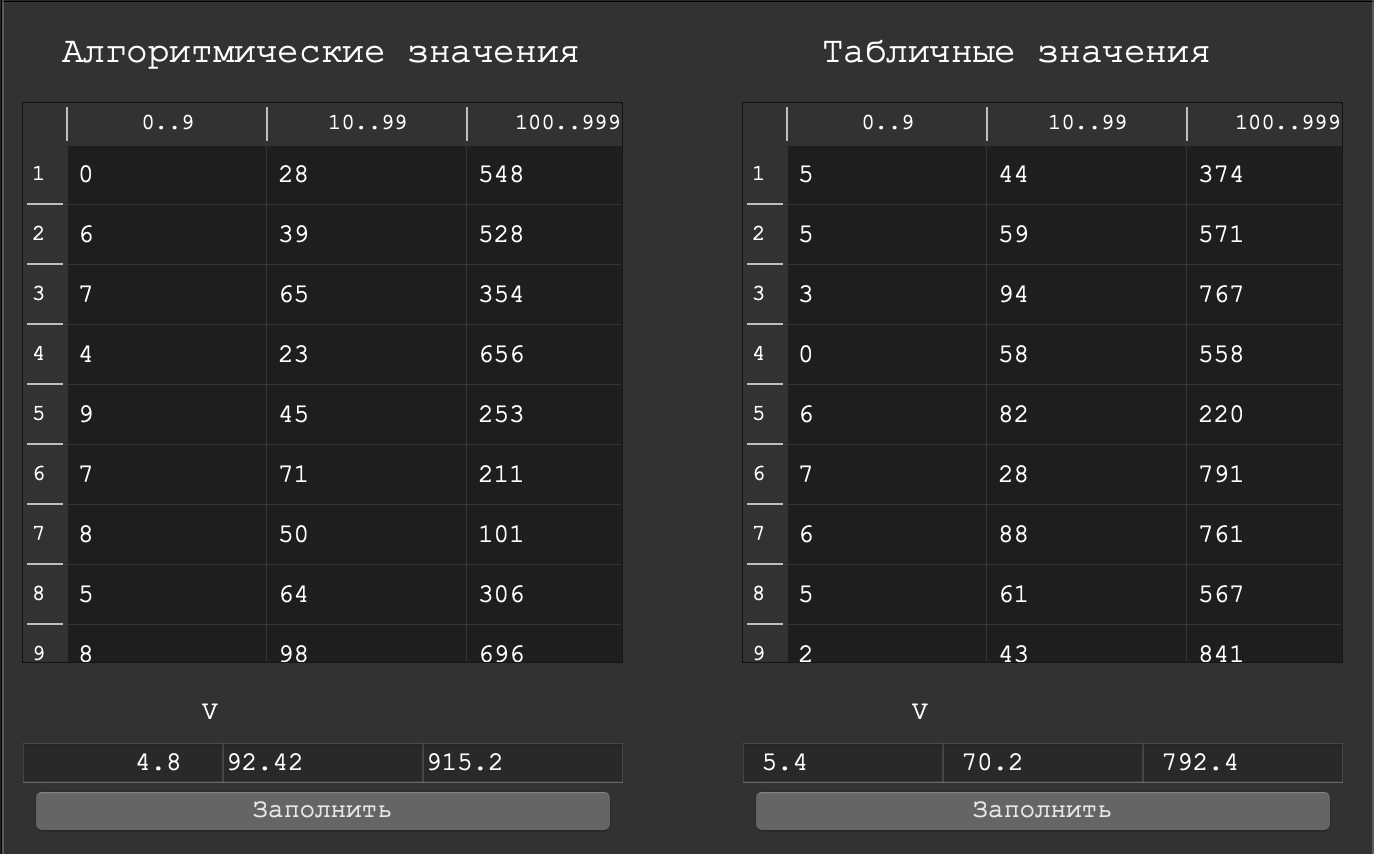
\includegraphics[width=\textwidth]{examples/1.png}
			\center{Пример №1 работы программы}
		\end{minipage}
		\begin{minipage}[b]{0.5\textwidth}
			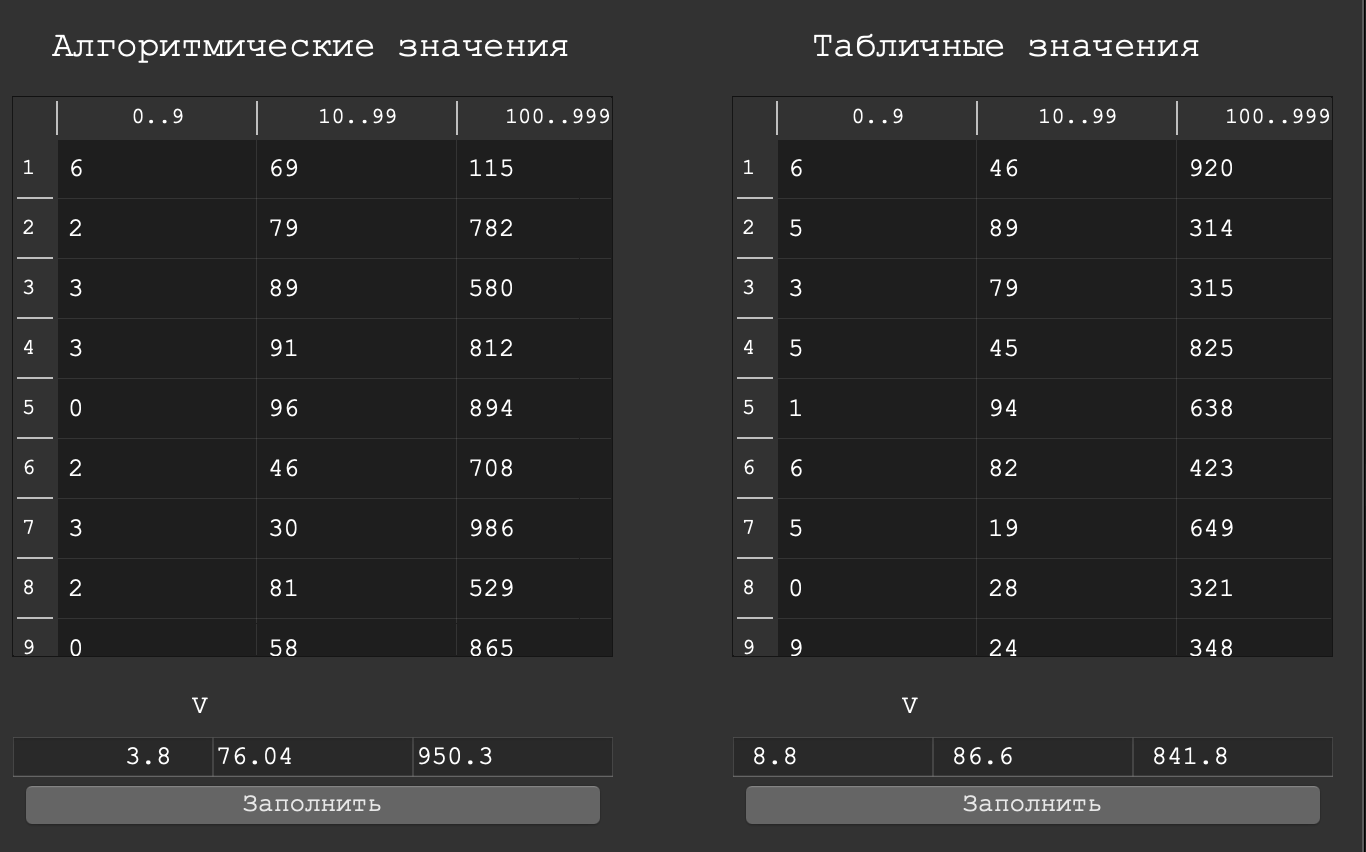
\includegraphics[width=\textwidth]{examples/2.png}
			\center{Пример №2 работы программы}
		\end{minipage}
		\label{ris:examples_1_2}
	\end{figure}

	\begin{figure}[h!]
		\begin{minipage}[b]{0.5\textwidth}
			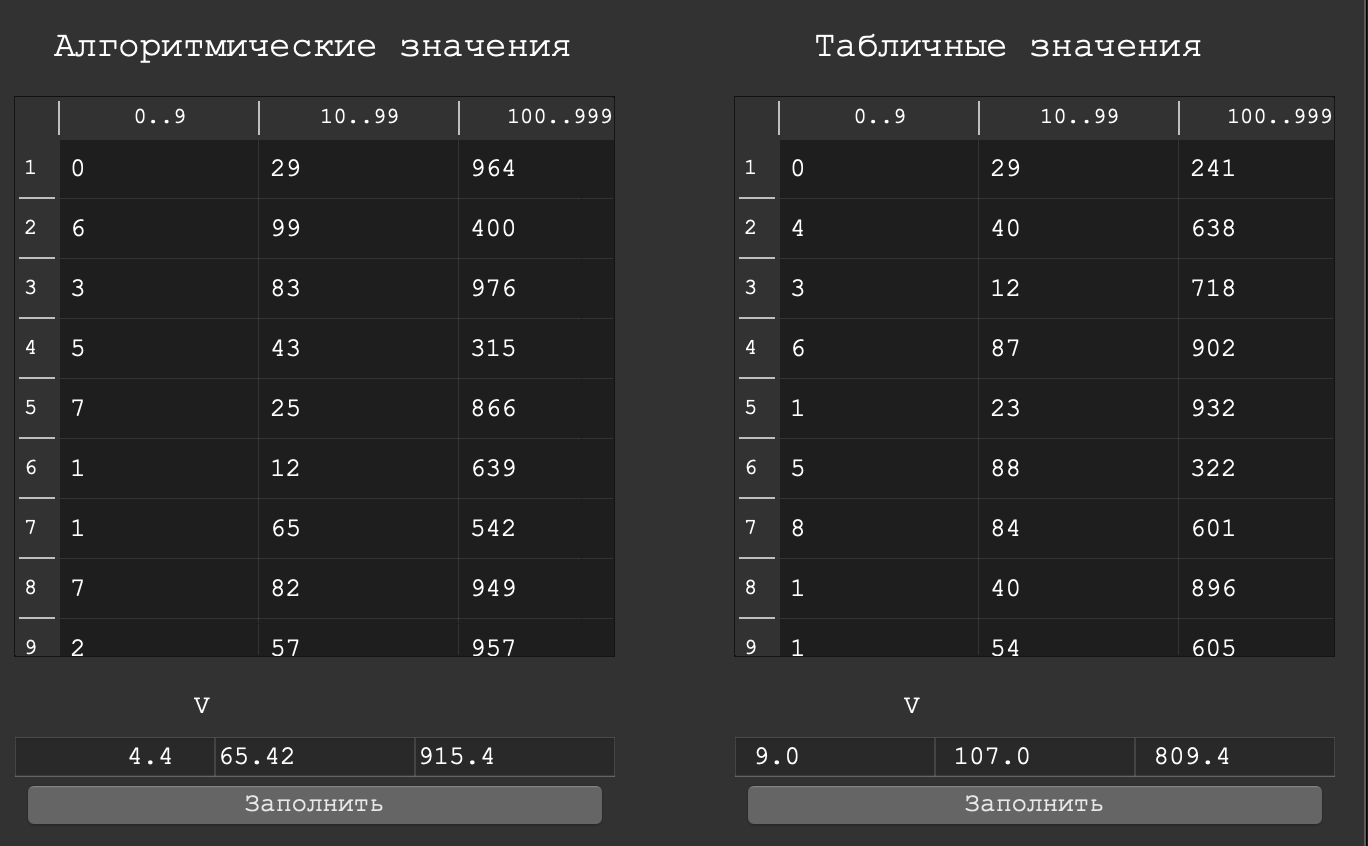
\includegraphics[width=\textwidth]{examples/3.png}
			\center{Пример №3 работы программы}
		\end{minipage}
		\begin{minipage}[b]{0.5\textwidth}
			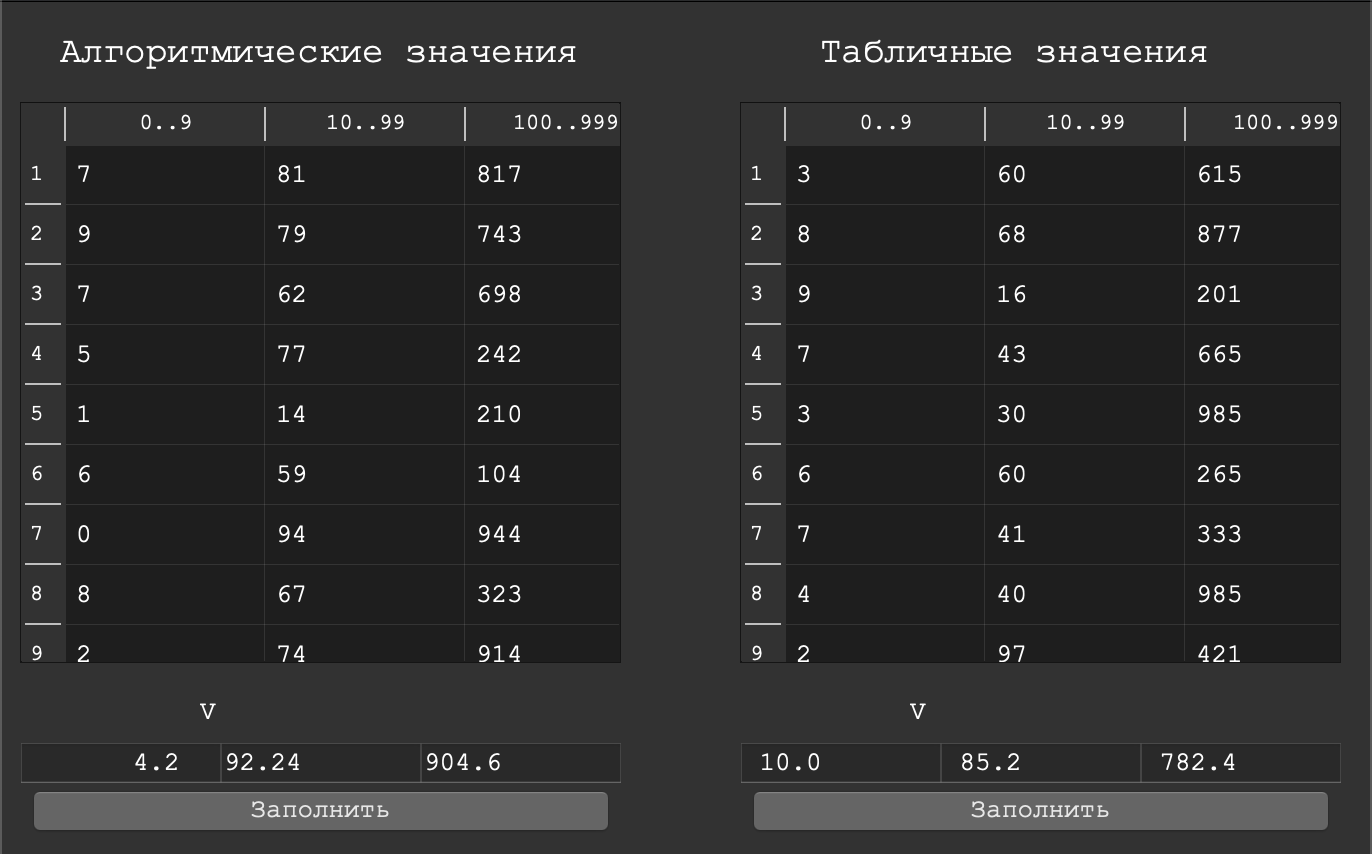
\includegraphics[width=\textwidth]{examples/4.png}
			\center{Пример №4 работы программы}
		\end{minipage}
		\label{ris:examples_3_4}
	\end{figure}
	
	\section*{Вывод}
	
	Исходя из приведенных результатов работы программы следует, что:
	\begin{center}
		\begin{longtable}[h!]{|p{0.05\linewidth}|p{0.12\linewidth}|p{0.12\linewidth}|p{0.12\linewidth}|p{0.12\linewidth}|p{0.12\linewidth}|p{0.12\linewidth}|}
			\hline
			{№} & {V (алг.) 0..9} & {V (алг.) 10..99} & {V (алг.) 100..999} & {V (табл.) 0..9} & {V (табл.) 10..99} & {V (табл.) 100..999}\\
			\hline
			{1} & {4.8} & {92.42} & {915.2} & {5.4} & {70.2} & {792.4}\\
			\hline
			{2} & {3.8} & {76.04} & {950.3} & {8.8} & {86.6} & {793.5}\\
			\hline
			{3} & {4.4} & {97.1} & {915.4} & {9.0} & {107.0} & {809.4}\\
			\hline
			{4} & {4.2} & {92.24} & {904.6} & {10.0} & {85.2} & {782.4}\\
			\hline
			\caption{}
		\end{longtable}
	\end{center}
	
	Сравнивая эти значения с значениями $V$ из таблицы 1, можно прийти к выводам, что вероятность $p$ при котором величина $V$ принимает указанные значения:
	
	\begin{center}
		\begin{longtable}[h!]{|p{0.05\linewidth}|p{0.12\linewidth}|p{0.12\linewidth}|p{0.12\linewidth}|p{0.12\linewidth}|p{0.12\linewidth}|p{0.12\linewidth}|}
			\hline
			{№} & {p (алг.) 0..9} & {p (алг.) 10..99} & {p (алг.) 100..999} & {p (табл.) 0..9} & {p (табл.) 10..99} & {p (табл.) 100..999}\\
			\hline
			{1} & {$<=25\%$} & {$<=75\%$} & {$<=75\%$} & {$<=25\%$} & {$<=25\%$} & {$<=1\%$}\\
			\hline
			{2} & {$<=25\%$} & {$<=50\%$} & {$<=95\%$} & {$<=75\%$} & {$<=50\%$} & {$<=1\%$}\\
			\hline
			{3} & {$<=25\%$} & {$<=75\%$} & {$<=75\%$} & {$<=75\%$} & {$<=95\%$} & {$<=5\%$}\\
			\hline
			{4} & {$<=25\%$} & {$<=75\%$} & {$<=75\%$} & {$<=75\%$} & {$<=50\%$} & {$<=1\%$}\\
			\hline
			\caption{}
		\end{longtable}
	\end{center}

	Видно, что при получении трехразрядных последовательностей с помощью таблицы случайных чисел при большом $n$ (10000) $V$ принимает такие малые значения, что вероятность $p$ стремится к 0. Другими словами, наблюдаемые значения очень близки к ожидаемым, что неудивительно, поскольку таблица случайных чисел по определению подразумевает, что это набор цифр такой, что вероятность возникновения любой цифры от 0 до 9 одна и та же ($p_s = \frac{1}{k}$).
	
	Также, заметим, что значения, сгенерированные алгоритмически, как и ожидалось, являются удовлетворительно случайными по отношению к $\chi^2$-критерию (в среднем $25\%<=p<=75\%$). Другими словами, $V$ достаточно большое, чтобы не считать результаты искусственными как в случае с табличным заполнением, но в то же время достаточно маленькое, чтобы считать результаты равномерно распределенными.
	
	Таким образом, полученные результаты полностью соответствуют ожидаемым.
	
	\newpage
	
	\addcontentsline{toc}{section}{Список используемой литературы}
	\begin{thebibliography}{2}
		\bibitem{mersen}
		Mersenne Twister: A 623-Dimensionally
		Equidistributed Uniform Pseudo-Random
		Number Generator [Электронный ресурс]. – Режим доступа: 
		https://citeseerx.ist.psu.edu/viewdoc/download?doi=10.1.1.315.6296\&rep=rep1\&type=pdf, 
		свободный – (10.10.2020)
		\bibitem{knut}
		Случайные числа [Электронный ресурс]. – Режим доступа: 
		https://vk.com/doc10903696\_194274866?hash=449e2b0813b76d81ce\&dl=db99c067f1ab31ac3b, 
		свободный – (10.10.2020)
	\end{thebibliography}
	
	
	
\end{document}
